\section{Efficiency of the soft muon tagger}

In this study we use the soft muon tagger (SLT) as a simple cut in the \ptrel distribution of
the muon and the Track Counting  as the two taggers of system8. System8 
requires the two taggers to be independent which means that the correlation 
coefficients between the tggers should be close to 1 in the System8. As we use 
the \ptrel information of the leading muon within the jet as our SLT tagger 
and the Track Counting as the Life Time tagger  which may use the muon track 
information for tagging, these correlation coefficients are deviated from 1.
We can solve this problem by using a the Track Counting tagger not involving 
the muon track. So we modify the Track Counting tagger such that it does not 
involve the muon track ( as discussed later ) and call it as the ``Modified 
Track Counting''. Figure~\ref{fig:Performanceplot} shows the performance plots
 comparing the modified Track Counting tagger with the Track Counting tagger
for the QCD RECO sample in the \pt range 80 to 120 GeV.

\begin{figure}[htbp]
  \begin{center}
    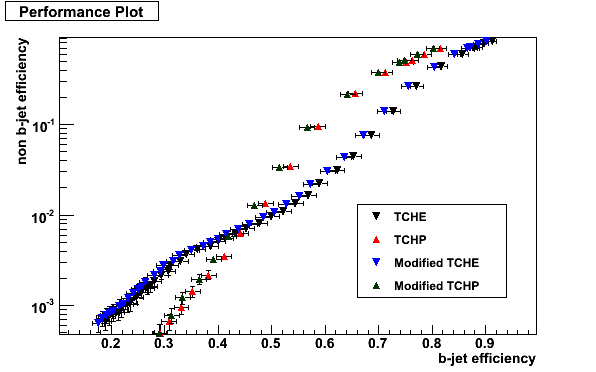
\includegraphics[width=120mm]{Figures/QCD_80_120.png}
  \end{center}
  \caption{Performance Plot comparing the performance of the default and 
modified Track Counting Algorithm for QCD 80-120 GeV sample.}
  \label{fig:Performanceplot}
\end{figure}


\subsection{Modified Track Counting}
\label{sec:MTC}
The Track Counting b-tagging method works as follows. For each selected track
in a jet, the impact parameter significance is computed. The jet is tagged if 
the number of tracks with an impact parameter significance exceeding a given 
cut is greater than a discriminator value.

To create a life time tagger not involving the muon track we modified 
the jet track associator. The Jet track associator  loops over all the jets 
in an event and associates the tracks to a jet if they lie within a cone of 
0.5. We modify the Jet track associator to look for the good muons using the
criteria.
\begin{itemize} 
\item   number of Hits in the track $ \ge $ 8;
\item   $\mu $ Pt $ \ge $ 6;
\item   normalized $\chi^{2} \le 5$,
\end{itemize}   
and reject the good muon tracks from the track collection and associate rest 
of the tracks to jets. The modified jets with no muon tracks are then used 
for Track Counting method giving a modified Track counting b-tagging algorithm.

The Modified Track Counting tagger can be used as one of the taggers of System8 
to determine the efficiency for the Soft Muon Tagger ( \ptrel).


